\chapter{Assignment \#7}
\label{ch:ass7n}

\begin{fullwidth}
\begin{enumerate}
\item Write a MATLAB user-defined function that determines the first derivative of a function that is given by a set of discrete points with equal spacing.  For the function name, use \lstinline[style=myMatlab]{yd = FirstDeriv(x,y)}.  The input arguments \lstinline[style=myMatlab]{x} and \lstinline[style=myMatlab]{y} are vectors with the coordinates of the points and the output argument \lstinline[style=myMatlab]{yd} is a vector with the values of the derivative at each point.  At the first and last points, the function should calculate the derivative with three-point forward and backward difference formulas, respectively.  At all other points, \lstinline[style=myMatlab]{FirstDeriv} should use the two-point centered difference formula.  Use \lstinline[style=myMatlab]{FirstDeriv} to calculate the derivative of the function given by the following tabulated data:

\begin{table}[h!]
\centering
\begin{tabular}{|c|c|c|c|c|c|}
\hline
$x$ & 1.1 & 1.2 & 1.3 & 1.4 & 1.5 \\ \hline
$f(x)$ & 0.6133 & 0.7822 & 0.9716 & 1.1814 & 1.4117 \\ \hline
\end{tabular}
\end{table}
Output the value of $\sfrac{df}{dx}$ at $x=1.3$.

\vspace{3.0cm}

\item Write a MATLAB user-defined function that calculates the second derivative of a function that is given by a set of discrete data points with equal spacing.  For the function name and arguments use \lstinline[style=myMatlab]{ydd = SecDeriv(x,y)}, where the input arguments \lstinline[style=myMatlab]{x} and \lstinline[style=myMatlab]{y} are vectors with the coordinates of the points, and \lstinline[style=myMatlab]{ydd} is a vector with the values of the second derivative at each point.  For calculating the second derivative, the function \lstinline[style=myMatlab]{SecDeriv} should use the finite difference formulas that have a truncation error of $\mathcal{O}(h^2)$.  Use \lstinline[style=myMatlab]{SecDeriv} to calculate the second derivative of the function that is given by the tabulated data below:

\begin{table}[h!]
\centering
\begin{tabular}{|c|c|c|c|c|c|c|c|c|c|c|c|c|}
\hline
$x$ & -1 & -0.5 & 0 & 0.5 & 1 & 1.5 & 2 & 2.5 & 3 & 3.5 & 4 & 4.5 \\ \hline
$f(x)$ & -3.632 & -0.3935 & 1 & 0.6487 & -1.282 & -4.518 & -8.611 & -12.82 & -15.91 & -15.88 & -9.402 & 9.017 \\ \hline
\end{tabular}
\end{table}
Output the value of $\sfrac{d^2f}{dx^2}$ at $x=2.5$.

\pagebreak

\item A radar station is tracking the motion of an aircraft.  The recorded distance to the aircraft, $r$, and the angle $\theta$ during a period of 60 seconds is given in the table below.  The magnitude of the instantaneous velocity and acceleration of the aircraft can be calculated by:
\begin{equation*}
v = \sqrt{\left(\frac{dr}{dt} \right)^2 + \left(r \frac{d \theta}{dt} \right)^2}, \ \ a = \sqrt{\left[\frac{d^2r}{dt^2} - r\left(\frac{d\theta}{dt} \right)^2 \right]^2 + \left[r \frac{d^2\theta}{dt^2} + 2 \frac{dr}{dt}\frac{d\theta}{dt} \right]^2}
\end{equation*}

Determine the magnitudes of the velocity and acceleration at the times given in the table.  Plot the velocity and acceleration versus time on the same plot with two different y-axes using the built-in MATLAB tool \lstinline[style=myMatlab]{yyaxis}. Calculate the derivatives using the \lstinline[style=myMatlab]{FirstDeriv} and \lstinline[style=myMatlab]{SecDeriv} functions you developed for the previous two problems.

\begin{table}[h!]
\centering
\begin{tabular}{|c|c|c|c|c|c|c|c|c|}
\hline
$t$ [s] & 0 & 4 & 8 & 12 & 16 & 20 & 24 & 28 \\ \hline
$r$ [km] & 18.803 & 18.861 & 18.946 & 19.042 & 19.148 & 19.260 & 19.376 & 19.495 \\ \hline
$\theta$ [rad] & 0.7854 & 0.7792 & 0.7701 & 0.7594 & 0.7477 & 0.7350 & 0.7215 & 0.7073 \\ \hline
$t$ [s] & 32 & 36 & 40 & 44 & 48 & 52 & 56 & 60 \\ \hline
$r$ [km] & 19.617 & 19.741 & 19.865 & 19.990 & 20.115 & 20.239 & 20.362 & 20.484 \\ \hline
$\theta$ [rad] & 0.6925 & 0.6771 & 0.6612 & 0.6448 & 0.6280 & 0.6107 & 0.5931 &0.5750 \\ \hline
\end{tabular}
\end{table}

\vspace{2.0cm}
\end{enumerate}
\end{fullwidth}

\begin{enumerate}[resume]

\item Write a user-defined MATLAB function to integrate a function $f(x)$ that is given in a set of $n$ discrete points using the trapezoidal rule.  Your function should \emph{not} require that the points be evenly spaced.  For the function name and arguments use \lstinline[style=myMatlab]{I=IntPointsTrap(x,y)}, where the input arguments \lstinline[style=myMatlab]{x} and \lstinline[style=myMatlab]{y} are vectors with the values of $x$ and the corresponding values of $f(x)$, respectively.  The output argument \lstinline[style=myMatlab]{I} is the value of the integral.  Use the function to estimate the surface area and volume of a wine barrel as illustrated in Figure \ref{fig:ass7n-prob4-fig}.  The diameter of the barrel is measured at the points provided in the table below.  The surface area, $S$, and volume, $V$, can be determined by:


\begin{marginfigure}
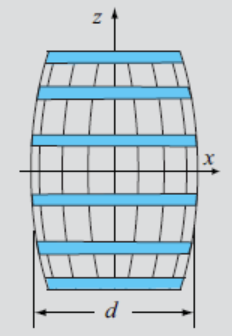
\includegraphics{ass7n-prob4-fig.png}
\caption{Schematic of wine barrel.}
\label{fig:ass7n-prob4-fig}
\end{marginfigure}

\begin{equation*}
S = 2 \pi \int_{0}^{L} r \ dz \ \ \text{ and } \ \ V = \pi\int_{0}^{L} \ dz
\end{equation*}
Your script should provide a properly formatted output of the surface area and volume of the barrel.
\end{enumerate}

\pagebreak

\begin{fullwidth}

\begin{enumerate}[resume]
\item Write a user-defined MATLAB function that uses Simpson's rule to integrate a function $f(x)$ that is given in a set of $n$ evenly spaced points.  For the function name and arguments use \lstinline[style=myMatlab]{I=SimpsonPoints(x,y)}, where the input arguments \lstinline[style=myMatlab]{x} and \lstinline[style=myMatlab]{y} are vectors with the values of $x$ and the corresponding values of $f(x)$, respectively.  The output argument \lstinline[style=myMatlab]{I} is the value of the integral.  Use the function to compute $\int_{0}^{1.8} f(x) \ dx$ with the tabulated data below:

\begin{table}[h!]
\begin{tabular}{|c|c|c|c|c|c|c|c|} 
\hline
$x$ & 0 & 0.3 & 0.6 & 0.9 & 1.2 & 1.5 & 1.8 \\ \hline
$f(x)$ & 0.5 & 0.6 & 0.8 & 1.3 & 2 & 3.2 & 4.8 \\ \hline
\end{tabular}
\end{table}
Your script should provide a properly formatted output of the value of the integral.

\vspace{3.0cm}

\item Write a user-defined MATLAB function to integrate a function, $f(x)$, in the domain $x \in [a,b]$, with five-point Gauss quadrature.  For the function name and arguments use \lstinline[style=myMatlab]{I=GaussQuad5ab(fun,a,b)}, where \lstinline[style=myMatlab]{fun} is a handle to the function that is being integrated, \lstinline[style=myMatlab]{a} and \lstinline[style=myMatlab]{b} are the lower and upper bounds of the integral, and \lstinline[style=myMatlab]{I} is the value of the integral.  Use the function to calculate the following integral:

\begin{equation*}
\int_{0}^{3} e^{-x^2} \ dx
\end{equation*}
Your script should provide a properly formatted output of the value of the integral.


\end{enumerate}
\end{fullwidth}




